For a quantum computer, multiple qubits are needed that are capable of interacting with each other. Thus, we need to make an array of the tweezers described in \cref{ch:tweezer}, spaced from each other in the order of micrometers. This can be done by sending different laser beams to the objective, all under slightly different angles. Experimentally, this can be realized by an \ac{AOD}: a device that diffracts light off of a sound wave in a crystal, where the degree of diffraction is controlled by a RF signal. By using 2 AODs in an orthogonal configuration, 2D Arrays can be realized \cite{Manuel2016}.

This chapter is on another method of making arrays of tweezers: the spatial light modulator. This device prints a hologram onto a laser beam, such that the interference pattern from this hologram in the focal plane of a lens yields any arbitrary array of spots. Spatial light modulators are thought to enable scaling to higher number of tweezers because when correctly used it can improve uniformity. In principle it is even possible to go make 3D arrays. 

\section{The Spatial Light Modulator}

The \ac{SLM} can manipulate properties of light like amplitude, phase and polarization. The type of SLM used is the phase-only SLM, and as the name suggests it can only control the phase of the light field. It does this by deploying a large array of pixels, where each individual pixel has a liquid crytal in it. The orientation of the crystal will change the refractive index because of the birefringence effect. The pixelated display is manufactured on a layer of silicon to address the voltage of each cell invididually. A sketch of the SLM pixels is shown in \cref{fig:LCoS}.

The working principle of this type of SLM has been documented extensively within our group, for example by \cite{Dijk2012,Bijnen2013,Bijnen2015}. 

\begin{figure}
    \centering
    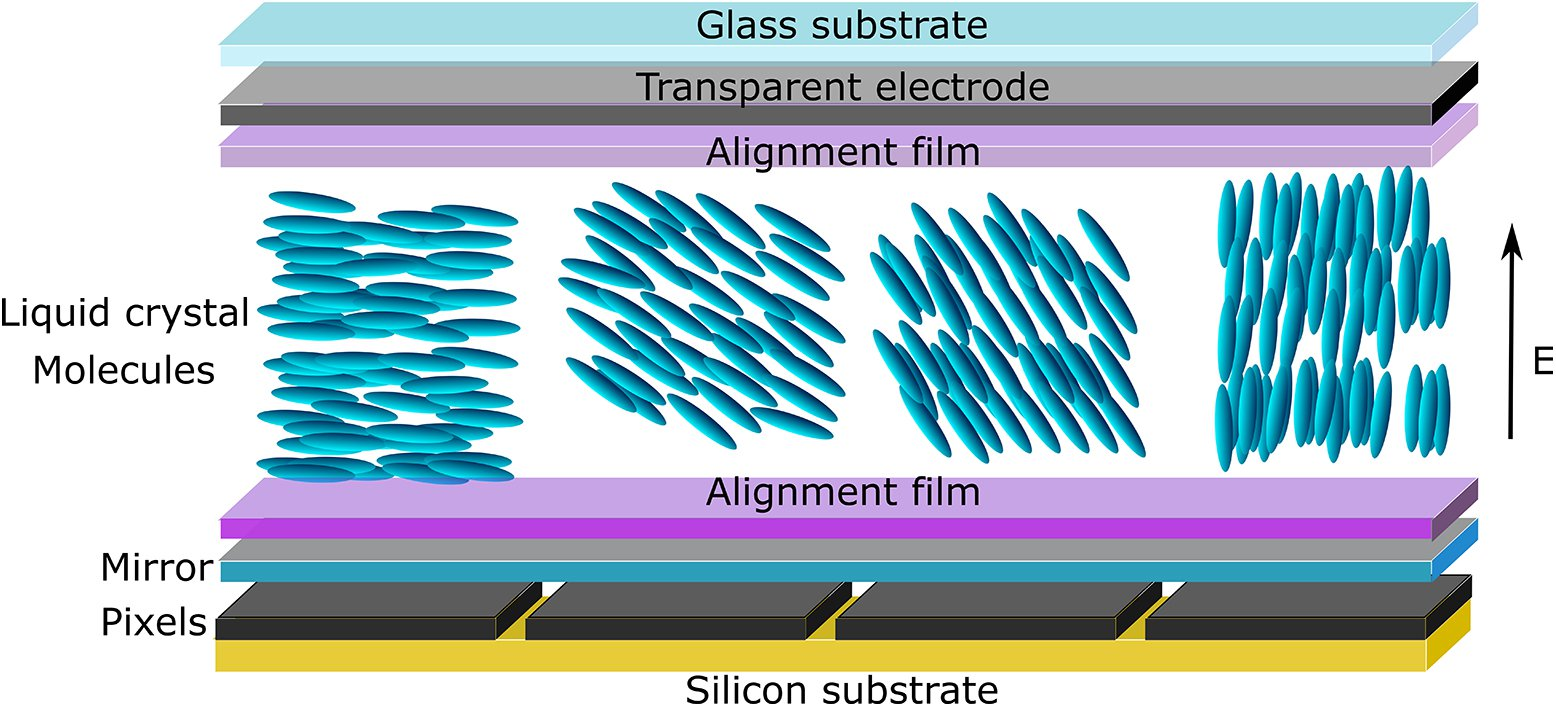
\includegraphics[width=0.6\linewidth]{figures/LCoS.png}
    \caption{The orientation of the liquid crystal cells changes as a function of the applied electric field $E$. Figure from \cite{Guzman2017}.}
    \label{fig:LCoS}
\end{figure}

\section{Phase Modulation}

In a phase only \ac{SLM}, each pixel can locally retard the field. As a result of diffraction, one can create arbitrary interference patterns in in the focal plane of the lens as shown by \cite{Bijnen2013}. The birefingence effect means the \ac{SLM} has two different refractive indices, somewhat confusingly called the ordinary and extraordinary refractive indeces respectively ($n_o$ and $n_e$). If the liquid crystal has a thickness $t$, the phase retardation will be $\phi_o = k t n_o$ and $\phi_e(V) = k t n_e(V)$ respectively, such that the phase retarder can be represented by the Jones matrix \cite{Guzman2017}

\begin{equation}\label{eq:JonesMatrix}
    M = e^{i \phi_0} 
    \begin{pmatrix}
        e^{i(\phi_e-\phi_o)} & 0\\
        0 & 1
    \end{pmatrix}
\end{equation}

Thus the phase retardance $\phi$ as a function of the applied voltage is \cite{Guzman2017}

\begin{equation}
    \phi(V) = \frac{2\pi}{\lambda} (n_e - n_0) t
\end{equation}

This proces can be done separately for each pixel, leading to a phase retardance $
\phi(x',y')$ where $x',y'$ are the coordinates in the plane of the SLM. When a laser beam with intensity $|U_i|^2$ impinges on the SLM, it will pick up a phase. Thus its field can be described as $U_i e^{i\phi(x',y')}$ this is shown in \cref{fig:SLMgeometry}. The field will interfere with itself, until at infinity (or in the focal plane of a lens) the distribution evolves to $|U_f|^2$.





\section{Finding the Hologram}\label{sec:IFTA}

We consider an ensemble consisting of the SLM and a perfect lens with focal length $f$. We define two cartesian coordinate systems: the SLM plane by $\{x',y'\}$ and the focal plane of the lens by $\{x,y\}$. The situation is sketched in \cref{fig:SLMLens}

We adapt the following notation, the \ac{SLM} plane, with individual pixels indexed by $j$, such that the coordinates are $x'_j, y'_j,0$ ($z'=0)$ because by definition the pixels lie in this plane. Next, we place a lens with focal length $f$ one focal length away from the SLM plane. One focal plane further is the focal plane of this Fourier lens, which we call the Fourier plane. See \cref{fig:SLMgeometry}. 

\begin{figure}
    \centering
    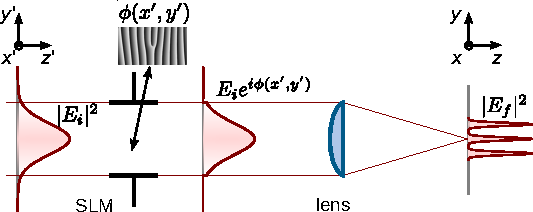
\includegraphics[width = 12cm]{figures/SLMfigure.pdf}
    \caption{Field with intensity distribution $|U_i|^2$ impinging on the SLM, which due to its finite size acts as an aperture. The lens makes the resulting image $|U_f|^2$ in its focal plane. Also shown: two cartesian coordinate systems in the SLM and focal plane. Not to scale. Adapted from \cite{Labuhn2016}.}
    \label{fig:SLMLens}
\end{figure}

When no phase is applied onto the SLM, the lens will focus all the light down to a diffraction-limited in the Fourier plane origin ($x=y=z=0$). As result of traveling from the $j$th pixel to the $m$th trap, under paraxial approximation, the light picks up a phase along the way of 

\begin{equation}
    \Delta_j^m = \frac{2\pi z_m}{\lambdaup f^2}(x_j^2+y_j^2)+\frac{2\pi}{\lambdaup f}(x_j x_m +y_j y_m)
\end{equation}

In the slm plane, we assume uniform illumination of the SLM such that the amplitude is the same $|U_i|$ everywhere. This may look like an unrealistic assumption considering we use a gaussian input beam, but we will see in a moment that in fact the input beam does not matter for the pattern produced. The SLM imprints a phase $\phi(x',y') = \phi_j$, such that the complex amplitude in the SLM plane for pixel $j$ is

\begin{equation}
    U_j(x',y') = U_j e^{i \phi_j}
\end{equation}

The contribution for the $m$th trap can be found by summing over all pixels, also keeping track of a phase factor in what is known as the diffraction formula:

\begin{equation}\label{eq:DiffractionFormula}
    \nu_m = e^{i k \left(2 f + z_m\right)}
    \frac{d^2}{i \lambda f} \sum_{j=1}^N e^{i(\phi_j - \Delta_j^m)}
\end{equation}

We assumed uniform illumination of the \ac{SLM}: $U_j =1$ everywhere. Furthermore $d$ is the pixel pitch of the SLM. But we are not interested in the phase of each in every spot, but only in the intensity. We will thus emit the prefactors in \cref{eq:DiffractionFormula} and normalize over $N$ pixels

\begin{equation}\label{eq:Vm}
    V_m = \frac{1}{N} \sum_{j} e^{i(\phi_j - \Delta_j^m)}
\end{equation}

While the algorithm works for 3D spot arrays, in this work we are primarily intersted in 2D arrays. Setting $z=0$ in \cref{eq:Vm} yields 

\begin{equation}
    V_m = \frac{1}{N} \sum_j \exp{\left(i\phi_j\right)} \exp{\left(
    - i 2\pi \left[
    \frac{x_m}{\lambdaup f} x_j + \frac{y_m}{\lambdaup f} y_j
    \right]
    \right)}
\end{equation}

Which is the 2D \ac{DFT} of $e^{i\phi}$ evaluated at spatial frequencies $x_m/\lambdaup f$ and $y_m/\lambdaup f$ in $x$ and $y$ respectively \cite{DiLeonardo2007,Bijnen2015}. The DFT can be efficiently evaluated on a computer using a \ac{FFT}. We stress that the FFT can only be used for 2D arrays. Thus in 2D, we have the following relation:

\begin{equation}
    V_m \propto \text{DFT}\left\{e^{i\phi(x',y'} \right\} 
    \left(x_m / \lambdaup f,y_m / \lambdaup f\right)
\end{equation}                                






\begin{equation}
    \centering
    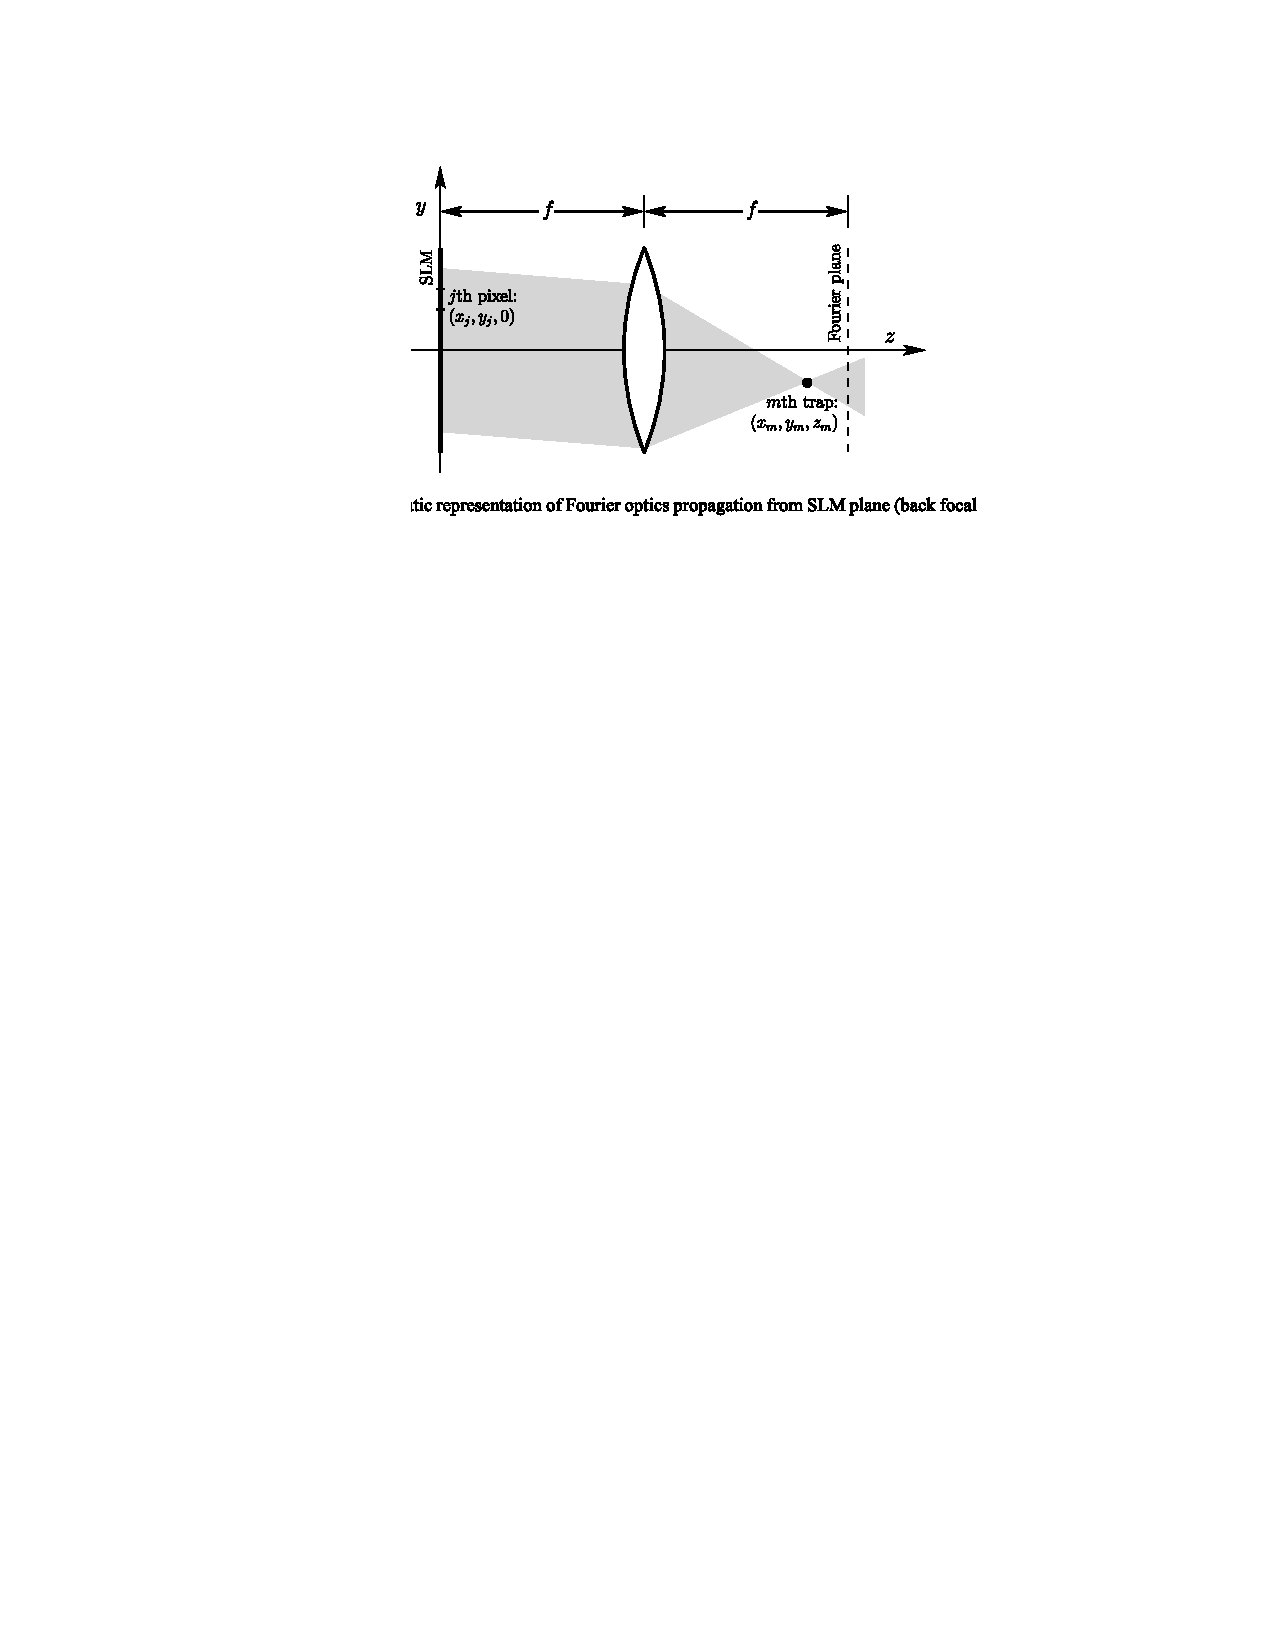
\includegraphics[width=0.\linewidth]{figures/SLMgeometry.pdf}
    %\caption{SLM and Fourier plane, each with their own coordinate labeling.}
    \label{fig:SLMgeometry}
\end{equation}





$U_f$ and $U_i$ are known in an experiment. Thus if one finds the right phase pattern or hologram $\phi(x,y)$, any intensity distrubution can be found from \cref{FourierLens}. But a single inverse inverse fast Fourier transform (IFFT) will not suffice, because this will not modulate the phase contributions of the invididual pixels $\phi_{kl}$ but also the amplitude contributions, which a phase-only SLM, by far the most commonly used SLM, cannot do. 

Instead, a set of algorithms known as inverse Fourier transform algorithms (IFTA) were pioneered by \cite{Hirsch1971} and adapted by \cite{Gerschberg1972} to tackle this task. The goal of the algorithm is to find a phase pattern for the SLM, such that in the focal plane of the lens, the light intensity $I_m = |V_m|^2$ in invidual spots $m$ is optimized in terms of parameters diffraction efficiency efficiency $e$ and uniformity of the spots $u$ \cite{DiLeonardo2007}:

\begin{equation}\label{EfficiencyUniformity}
    e = \sum_m |V_m|^2, \quad u= 1-\frac{\text{max}(|V_m|^2)-\text{min}(|V_m|^2)}{\text{max}(|V_m|^2)+\text{min}(|V_m|^2)}
\end{equation}

These are theorical quantities and not actually measured. The algorithm works essentially by virtually propagating light back and forward in iterations acoording by computing FFT and IFFT's, applying constraints in the focal and SLM plane in each iteration. 




In order to overcome this issue, after the inverse FFT we replace the computed complex amplitude by our incident amplitude $PU_0$ and we compute its FFT, returning again to the focal plane. Here, we replace the obtained obtained complex amplitude for the desired amplitude $|U(x,y)|^2$. This process is iterated several times until convergence is reached. This family of algorithms is refered to as an inverse Fourier transform algorithm (IFTA) and essentially consists of virtually propagating light back and forward between the input and focal planes. 

IFTA algorithms were pioneered in\cite{Hirsch1971} and adapted for phase retrieval by \cite{Gerschberg1972}. The implementation of the IFTA algorithm was done by \cite{Bijnen2013,Bijnen2015}. It was adapted to achieve better convergence by defining a signal window, within it the desired pattern is made. Outside of this window, the amplitude is unconstrained. This relaxiation of constraints allows for better convergence of the desired pattern, at the cost of energy lost outside of the window \cite{Bijnen2013,Bijnen2015}.

\section{Operating the SLM}

The algorithm as explained in \cref{IFTA} was implented in software by \cite{Bijnen2015}. The input intensity $|PU_0|^2$ is assumed to be a plane wave. Using the SLM is explained here. The SLM will inevitably lose power due to several processes. These are explained here. 

\subsection{Diffraction}

Diffraction. The SLM is a device consisting of individual pixels. Therefore, it is essentially a 2D diffraction grating, and light will diffract in several directions. In 1D, we know that according to diffraction theory the diffraction angle maxima $\theta_m$ from a plane wave incident at $\theta_i$ occur at $\theta_m = \arcsin(\sin\theta_i - m\lambdaup/d)$, where $m$ is the order of diffraction and $d$ the pixel pitch. We are interested in the light in the $m=0$ diffracton order, other orders are spatially filtered out and unused.

\subsection{Zeroth Order}

Light can reflect on the spacings between the pixels. Also, it can reflect off of the electrodes at the back of the device. All of this undiffracted light is focussed onto the optical axis by the objective. As a result, the optical axis unusable to shape light and we have to seperate our modulated light from this 'zeroth order peak'. This is done by superimposing a linear phase on top of the SLM phase pattern. Because the phase is computed modulo 2$\pi$ the resulting pattern is a blazed grating. Light from the higher diffraction orders and zeroth order peak can be blocked by an iris in the focal plane of an intermediaty lens. 
    
\subsection{Finite aperture size}

In order to employ the maximum amount of pixels the SLM has to offer, and therefore the maximum drawing area in the focal plane of the Fourier lens, all of the pixels should be illuminated. However, because the incident beam is described by a gaussian, this will lead to power loss as a result of light not falling on the active pixel area. 
    
We can estimate this power loss by shining a Gaussian beam $G(x,y)$ of width $w(z)$ and power $P_0$ onto a rectangular aperture of dimensions $(2S_x, 2S_y)$ where $S_{x,y}$ are the semi-widths of the aperture. The relative power transmission $P/P_0$ can be found by integrating the intensity of the beam \cref{GaussianBeamIntensity} in cartesian coordinates over the aperture

\begin{equation}\label{RectAperturePower}
    \frac{P}{P_0} =
    \iint I(x,y) dA=
    \text{Erf}\left(\frac{\sqrt{2}S_x}{w(z)}\right) \text{Erf}\left(\frac{\sqrt{2}S_y}{w(z)}\right)
\end{equation}

where Erf($\cdot$) denotes the error function. The optimum incident beam size $w(z)$ is thus a compromize between drawing area and power efficiency. We chose $w(z) \approx S_{x}$, specifically $w(z) = 4.8$ mm and $S_x = 4.9$ mm. 

\subsection{Reflectivity}

As can be seen in \cref{fig:LCoS}, the light will back reflect at after passing through the liquid crystal. This back plate will have a non-perfect anti relection coating, leading to some light being absorbed. 


\section{Calibration}

We know that the phase pattern of the SLM is realized by the birefringence effect. However, it turns out the phase retardation as a function of the applied voltage is non-linear. Additionally, the surface of the SLM is not fully flat, introducing a small aberration. Both of these effects differ for indiviual SLM units, even for the same model. Therefore, here we will briefly review how to calibrate the SLM to account for these two effect.s 

\subsection{Electro-Optic Response}

The goal of the calibration of the phase as a function of applied voltage (electro-optic response) is to 

\begin{enumerate}
    \item Achieve a linear electric-optic response. 
    \item Ensure the phase is modulate by a full wave $2\pi$ spanning the minimum to the maximum grey level. 
\end{enumerate}

\subsection{Optical flatness correction}

Because of the silicon producetion process, the chip is not completely flat. The optical flatness of SLM was measured to be $0.18\lambdaup$ by manufacturer Meadowlark. Additionally, the manufacturer measured the shape of the correction using Michelson interferometry. By substracting this measured non-flatness from the calculated phase pattern, this effect can be corrected. 


\section{Arrays of tweezers}

\subsection{Array Spacing}

Because of the properties of the Fourier transform, the smallest possible 

\subsection{Spot Detection}

We make an arbitrarily sized array of optical tweezers. For detecting maxima locations, we could simply set pixels above a certain count threshold as a maxima. The disadvantage of this is that a noisy pixel could be detected as a spot, which would hinder analysis. 

To combat this, we first convolute the image with a Laplacian of Gaussian filter, which first smoothes the image to reduce noise. Subsequently it computes the 2D laplacian to detect edges. If this second derivative is above a certain threshold, we detect the edge as a spot. If the detected amount of spots is not the expected amount, we can easily tune the threshold. The camera image is cropped into regions of interest around the spots marked by the Laplacian of Gaussian filter. 

\subsection{Spot Fitting}

Our tweezers should be described by \cref{FourierBesselAperture}. However, because of a lack of an analytic expression this is not the most convenient. \cref{FourierBesselAperture} can closely be resembled by a Gaussian. We will therefore use the following function for fitting spots numbered $k$

\begin{equation}\label{2DGaussian}
    G_k(x,y) = U_k \exp{\left(-\frac{(x_k-x_{k,0})^2}{2\sigma_{k,x}^2}\right)}
    \exp{\left( \frac{-(y_k-y_{k,0})^2}{2\sigma_{k,y}^2} \right)}
\end{equation}

Here $U$ is the 'trap depth', $x,y$ are the cartesian coordinates in the camera frame and $x_0,y_0$ is the center of the spot. Lastly $\sigma_{x,y}$ are standard deviations in $x$ and $y$. In principle, because the limiting aperture in the system is a circular aperture, the spots should be more or less symmetric and $\sigma_x\approx \sigma_y$ which we confirmed. We find the $1/e^2$ waist $w_k=\sigma_{k,x}+\sigma_{k,y}$. 